\documentclass[journal]{IEEEtran}
\usepackage{amsmath,amssymb}
\usepackage{booktabs}
\usepackage{graphicx}
\usepackage{hyperref}

% ---- Anonymization toggle: keep in sync with draft.tex ----
\newif\ifanonymous
\anonymoustrue

\begin{document}

\title{Supplementary Material for\\ Diagnosing and Repairing Out-of-Distribution Failure\\ in MOBA Draft Policies}
\ifanonymous
\author{Anonymous Authors}
\else
\author{Max~Segan, Ernest~Pysher, James~Frankel, and Hod~Lipson}
\fi
\maketitle

\section{Fused CUDA Kernels for MCTS Training}
\label{sec:cuda}

The MCTS training campaign in the main paper, 195 complete training runs spanning simulation budgets up to 800 per move and episode counts up to 1M, was only feasible because of the fused CUDA implementation described here. AlphaZero-style MCTS training is computationally demanding: each episode requires $\sim$8 MCTS searches of 200 simulations each, with a neural network forward pass at every leaf node. Standard implementations incur Python interpreter overhead, CUDA kernel launch latency, and host-device synchronization for each of the $\sim$3,200 forward passes per episode.

We developed a fused CUDA implementation that runs entire MCTS episodes inside a single kernel launch. One thread block (256 threads) executes one complete draft episode: thread~0 drives all sequential logic (UCB selection, action sampling, backpropagation) while all 256 threads cooperate on matrix multiplications during neural network forward passes via shared memory. The forward pass functions (\texttt{linear\_layer}, \texttt{batchnorm\_relu}, \texttt{residual\_block}) are compiled as \texttt{\_\_device\_\_} functions callable from within the kernel with zero launch overhead. Two additional optimizations compound with the fused kernel:
\begin{itemize}
    \item \textbf{Split backbone from heads}: Value symmetrization runs only the small value head (257$\to$128$\to$64$\to$1) twice rather than the full backbone, halving symmetrization cost.
    \item \textbf{Pipelined generation}: Episode results are written into pre-allocated ring buffers via C++ \texttt{memcpy}; a generation thread launches GPU batches asynchronously while the main thread performs gradient updates.
\end{itemize}

\begin{table}[t]
\centering
\caption{MCTS training throughput across implementation stages.}
\label{tab:throughput}
\begin{tabular}{lcc}
\toprule
Implementation & ep/s & Bottleneck \\
\midrule
Python + PyTorch CPU & 1.2 & Forward pass dispatch \\
C++ tree, batched virtual loss (K=32) & 5.1 & Amortized sync \\
Full CUDA kernel (1 block=1 ep) & 26 & Python buffer overhead \\
+ ring buffer + pipelining (bring-up) & 50 & Warm-up, small batches \\
Final (steady state, campaign) & \textbf{140} & GPU compute \\
\bottomrule
\end{tabular}
\end{table}

Table~\ref{tab:throughput} shows the progression; all stages measured at 200 simulations per move. The first four rows are development-time measurements taken as each optimization landed; the final row is the sustained steady-state rate of the finished implementation, measured across the full training campaign (195 complete runs, 128 concurrent episodes per kernel launch) under four-GPU load on NVIDIA RTX PRO 6000 Blackwell Workstation Edition GPUs (96~GB each). Uncontended single-run throughput reaches 190 episodes/second. Two corrections to earlier versions of this table: an earlier draft printed 10.9 ep/s for the virtual-loss stage, but 10.9 was the development log's speedup \textit{factor} over the sequential Python pipeline (2{,}145 vs.\ 197 ms/episode); the rate is 5.1 ep/s, and since the C++ engine was virtual-loss batched from its first commit, the two development rows collapse to one. The rows are also heterogeneous in leaf evaluation (development history, not a controlled comparison); the controlled comparison appears below. The gap between the bring-up and final figures reflects cumulative-average warm-up in early measurements and subsequent batching maturity. Sustained throughput is 117$\times$ the Python baseline and scales inversely with simulation budget (74 episodes/second at 400 simulations per move), confirming the implementation is compute-bound rather than overhead-bound: a 300K-episode run completes in under 40 minutes on one GPU. Each episode requires $\sim$1~MB of global memory for the MCTS tree (2,048 nodes); with 128 concurrent episodes per kernel launch, total GPU memory usage is $\sim$140~MB plus 10~MB of network weights.

\paragraph{Apples-to-apples baseline.} For a controlled speedup claim we built a tuned host-tree baseline in the style of KataGo's batched-evaluation pipelines: 64--256 CPU threads each running one episode's tree, leaf evaluations batched across threads onto the GPU via cuBLAS GEMM over multiple streams, reproducing the production kernel's exact per-simulation work (policy priors at expansion, Generic Draft rollout to terminal at every leaf, symmetrized enriched-WP scoring). At equal work \textit{and} equal search semantics (leaf batch 1; first-turn root-visit total-variation distance from the kernel 0.047, at the 0.044 kernel-vs-kernel seed-noise floor; win rate vs.\ GD 0.761 vs.\ the kernel's 0.757), the host pipeline sustains 68 ep/s against the fused kernel's 151 ep/s on the same GPU: the fused kernel is 2.2$\times$ faster, the figure quoted in the main paper, because per-simulation host-device round trips cannot be amortized without within-episode leaf batching. Virtual-loss leaf batching does push the host pipeline to 163 ep/s (1.07$\times$ the kernel), but only by degrading the search itself: at leaf batch 32 the win rate vs.\ GD falls from 0.757 to 0.531 and the visit-distribution TV rises to 0.62; softening virtual loss to 0.25 recovers only 0.712.\footnote{The equivalence check also uncovered a virtual-loss bookkeeping bug in the historical batched implementation of Table~\ref{tab:throughput}: the virtual-loss undo was applied to the root node as well as the descended path, driving the root visit count negative, at which point $\sqrt{\smash[b]{\text{negative}}}=\text{NaN}$ poisoned UCB selection from the second leaf batch onward.} Per-component profiling shows the GD rollout evaluation dominates ($\sim$75\% of the host pipeline's evaluator wait time; policy priors and WP scoring share the rest), and that the kernel's per-node cache of opponent GD distributions is dead code in practice: leaves expand only at our-team steps, so cached nodes are never re-traversed at opponent steps (measured cache-miss count 0), which is why it is not listed among the optimizations above. The remaining advantages of the fused kernel are operational: 0.12~s startup, a deterministic $\sim$270~MB footprint, and no host thread pool or Python runtime at inference.

\section{Synthetic Augmentation Sweep: Unseen vs.\ Sparse Scope}

The main paper's synthetic-data repair swept 27 configurations varying
augmentation win rate (10/20/30\%), volume (50/100/200 per composition
per tier), and scope (unseen only, sparse low-WR only, or both).
Augmenting unseen compositions is the active ingredient. At the best
volume (100) and WR (10\%), sparse-only augmentation (reinforcing
compositions with $<$300 games and $<$48\% WR) leaves the 5-tank
pathology unrepaired (WP 0.23, vs.\ 0.15 for the unaugmented baseline),
while unseen-only augmentation drives it to 0.07; the ``both'' scope is
intermediate (0.11).

\section{Validity of the Interaction Metrics}
\label{sec:metricvalid}

\begin{figure}[t]
\centering
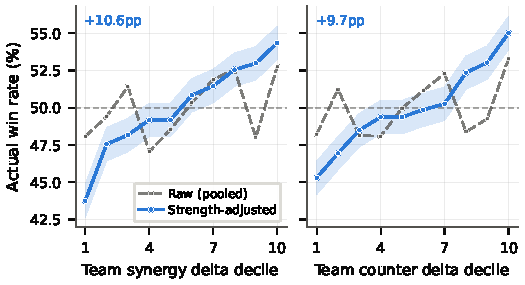
\includegraphics[width=\columnwidth]{fig_metric_validation.pdf}
\caption{Actual win rate vs.\ interaction-metric decile on the held-out test split (38{,}981 replays, both sides, 77{,}962 team observations; shaded: 95\% binomial CI). Gray: pooled deciles. Blue: strength-adjusted deciles, computed within strata of skill tier $\times$ own-team $\times$ opposing-team mean hero win rate quintiles and count-weighted across strata.}
\label{fig:metricvalid}
\end{figure}

The main paper's interaction-awareness metrics are built from the pairwise synergy and counter deltas (Section~III of the main paper), which subtract from each observed pair win rate an independence expectation formed from the two heroes' individual win rates. We validate that these deltas carry real outcome signal on the held-out test split, scoring each side of each test draft with the exact metric implementations and frozen statistics used throughout, against the game's actual outcome. Pooled naively (gray in Fig.~\ref{fig:metricvalid}), the decile curves are \textit{not} monotone, and this structure is systematic rather than noise: the enriched WP model's predictions reproduce it. The cause is the metrics' own construction: subtracting the individual-strength expectation makes the deltas strongly anti-correlated with team hero strength ($r = -0.87$ between team synergy delta and team mean hero win rate), so teams of individually strong heroes regress toward the mean, receiving negative deltas while still winning more. Controlling for exactly that component, deciles within tier and own/opposing team-strength strata (blue), both metrics are cleanly monotone in actual win rate: bottom-to-top-decile spreads of $+10.6$pp for team synergy delta (43.8\% $\to$ 54.3\%, 9/9 decile steps increasing) and $+9.7$pp for team counter delta (45.3\% $\to$ 55.0\%, 8/9 increasing), with $\pm$1.1pp CIs. The interaction deltas thus measure a real, outcome-relevant property of a composition beyond individual hero strength, which is precisely the component they are designed to isolate.

\section{Dual-Snapshot Stability of the Interaction Metrics}
\label{sec:dualsnap}

The main paper notes (Section~III) that the interaction-metric magnitudes are snapshot-sensitive: re-pulling the community aggregate statistics shifts the pairwise deltas systematically, so absolute synergy and counter values are not comparable across snapshots. The collapse diagnosis and the method comparisons rest instead on \textit{relative} gaps. Here we verify directly that the relative ordering of strategies is stable across statistics snapshots.

The twelve MCTS training configurations of the main paper's simulation-scaling study were each re-benchmarked twice under an identical protocol (15 seeds $\times$ 600 drafts against behavioral-cloning opponents): once with the aggregate statistics in use before the May 2026 re-pull, and once with the frozen 2026-05-19 snapshot used throughout the paper. The trained policy networks are identical in both arms; only the statistics feeding the enriched features and the metric lookups change. Table~\ref{tab:dualsnap} shows synergy exploitation and counter responsiveness per configuration under both snapshots.

\begin{table}[t]
\centering
\caption{Interaction metrics for twelve MCTS configurations under two statistics snapshots (earlier pull vs.\ frozen 2026-05-19; 15 seeds $\times$ 600 drafts each, identical policies). Rows sorted by frozen-snapshot synergy. Spearman rank correlation of the configuration ordering across snapshots: $\rho = 1.00$ (synergy), $\rho = 0.97$ (counter), $\rho = 1.00$ (early resilience, not shown).}
\label{tab:dualsnap}
\begin{tabular}{lcccc}
\toprule
& \multicolumn{2}{c}{Synergy} & \multicolumn{2}{c}{Counter} \\
\cmidrule(lr){2-3}\cmidrule(lr){4-5}
Config & Earlier & Frozen & Earlier & Frozen \\
\midrule
L\_800sim\_4M & $+$1.20 & $+$1.21 & $+$0.19 & $+$0.18 \\
J\_800sim & $+$1.07 & $+$1.07 & $+$0.20 & $+$0.20 \\
I\_600sim & $+$0.99 & $+$1.01 & $+$0.20 & $+$0.19 \\
F\_400sim & $+$0.92 & $+$0.94 & $+$0.18 & $+$0.19 \\
E\_1M & $+$0.91 & $+$0.94 & $+$0.18 & $+$0.18 \\
H\_augmented & $+$0.73 & $+$0.75 & $+$0.16 & $+$0.16 \\
B\_fullwp & $+$0.69 & $+$0.73 & $+$0.15 & $+$0.15 \\
A\_partial & $+$0.68 & $+$0.72 & $+$0.14 & $+$0.14 \\
K\_truebase & $+$0.54 & $+$0.59 & $+$0.13 & $+$0.12 \\
G\_base & $+$0.53 & $+$0.57 & $+$0.11 & $+$0.11 \\
C\_large & $+$0.45 & $+$0.49 & $+$0.13 & $+$0.13 \\
D\_deep & $+$0.14 & $+$0.14 & $+$0.12 & $+$0.11 \\
\bottomrule
\end{tabular}
\end{table}

The ordering is essentially unchanged: Spearman rank correlations across the twelve configurations are 1.00 for synergy, 0.97 for counter responsiveness (adjacent reshuffling among near-tied configurations), and 1.00 for early-pick resilience. Absolute values shift by at most $+$0.05 (synergy) and $\pm$0.007 (counter), small relative to the between-configuration gaps the paper's conclusions rest on (e.g., the $+$0.9 synergy separation between deep-search and anchored strategies). This benchmark predates the paper's final retrained models, so its absolute magnitudes differ from the main-paper tables; the comparison isolates the snapshot effect, which is the quantity of interest. Strategy-level rich evaluations (Table~IV of the main paper) were run only under the frozen snapshot; the earlier pull existed as a live database state and was not retained, so the controlled dual-snapshot evidence above is the MCTS configuration family, which spans the full range of interaction-awareness the paper reports.

\section{External Validation on Coordinated-League Drafts}
\label{sec:ngs}

The main paper's behavior policy is uncoordinated ranked-ladder play, and its Limitations note that every evaluation shares that corpus. As an external test, we evaluate the frozen snapshot-trained win-probability models on drafts from the Nexus Gaming Series (NGS), an amateur organized league in which persistent five-player teams draft together with dedicated captains. Scanning the Heroes Profile NGS archive yielded 11{,}132 games, of which \textbf{11{,}034} pass filtering (patch 2.55, complete 16-step draft, known winner), spanning 2021--2026 across ten season clusters, the same patch era as our ladder corpus.

\paragraph{Coordinated drafts are \textit{more} meta-concentrated.} A natural hypothesis is that coordinated teams, freed from solo-queue comfort picking, explore more of the hero pool. The data show the opposite, at both the hero and the composition level. Hero level: NGS pick entropy is 5.92 bits vs.\ the ladder's 6.25 (effective pool 60.5 vs.\ 75.9 heroes), the top-10 heroes take 33.5\% of picks vs.\ 25.1\%, and the off-meta share (picks outside the ladder top-30) is 39.8\% vs.\ 43.3\%; hero pick-rate rank correlation between the populations is 0.74. Composition level: NGS fields 78 distinct role compositions vs.\ 238 on ladder, with composition entropy 2.69 vs.\ 3.06 bits, the top-5 compositions covering 84.3\% vs.\ 78.6\% of teams, and 90\% coverage reached in 9 vs.\ 12 compositions. The modal composition is the same standard core in both populations (bruiser/healer/double-ranged/tank: 53\% vs.\ 50\%); NGS's second-most-common composition is a double-tank variant (12.3\%). Our reading: coordinated teams converge on a known-good playbook, while ladder ``diversity'' partly reflects uncoordinated comfort picking and error. This corroborates the main paper's characterization of the behavior policy as shaped by social dynamics rather than win maximization: removing the coordination constraint is not what diversifies drafting; removing strategic discipline is.

\paragraph{Win-probability transfer.} Scored at the game level with symmetrized predictions, the enriched model reaches 55.5\% accuracy on NGS (95\% binomial CI [54.6\%, 56.4\%]) against 58.1\% on held-out ladder data; the naive and augmented variants score 55.3\% and 55.5\% (CIs $\pm$0.9pp at this sample size, sufficient to bound the ladder-to-NGS change). The degradation is localized where the shift is largest: splitting NGS drafts into quartiles by off-meta pick share, the enriched model scores 57.6\% on the most-meta quartile, essentially its ladder accuracy, falling to 54.5\% on the least-meta quartile. Calibration degrades mildly for the feature-based models (enriched ECE 0.0165 on NGS vs.\ 0.0050 on ladder; the naive model stays well calibrated at 0.0063). Notably, 99.98\% of NGS team compositions fall within the composition sets observed in the ladder-era aggregate statistics, so this shift is a re-weighting within familiar structures, not entry into the never-observed region that the paper's synthetic augmentation targets. One caveat caps interpretation: NGS outcomes also reflect persistent team-strength imbalances that the models never observe (the same organized teams meet repeatedly), which lowers attainable accuracy in a way not directly comparable to solo-queue ladder play.

\section{Draft Concentration and Out-of-Distribution Extrapolation}
\label{sec:concentration}

The main paper's Limitations name its central vulnerability: every adjudication, including the tournament, is scored by value functions trained on the authors' own corpus, so a policy that drifted into states where those functions are systematically wrong could be graded a winner exactly where it deserves to lose. This section measures how far the winning agent actually drifts. The finding: the agent concentrates onto a small hero pool whose individual, pairwise, and trio advantages are directly verifiable in real game outcomes, and it leaves the data only at the level of exact five-hero compositions, while staying inside role structures the 9M-game aggregates validate. Its out-of-distribution exposure is narrow and characterizable. All measurements below use a fixed diagnostic protocol (200 drafts per seed, mid tier, 200 inference simulations, symmetrized enriched judge); per-configuration tables ship with the release repository.

\paragraph{Concentration is method-wide, search-aligned, and value-model-independent.} Under the headline J\_800sim configuration, all 15 seeds share the identical top-3 pick set \{Hogger, Samuro, Rehgar\}; a single seed uses 25.3$\pm$2.1 distinct heroes at 3.65$\pm$0.10 bits of pick entropy, and pooling all fifteen seeds adds only +0.09 bits (36 distinct heroes): the seeds converge on one head, not fifteen different ones. Deeper search does not concentrate further (per-seed entropy 3.62$\to$3.65 bits from 200$\to$800 training simulations, judge WP 0.726$\to$0.768), but longer training does: two diagnostic training lengths added to the main paper's grid (100K and 500K episodes, 200 simulations, 5 seeds each) complete the curve 100K$\to$300K$\to$500K$\to$1M episodes as entropy 3.84$\to$3.62$\to$3.37$\to$3.34 bits per seed against judge WP 0.688$\to$0.726$\to$0.744$\to$0.752 and degenerate rate 19.3$\to$11.0$\to$4.7$\to$5.4\%: the 100K policy is the most diverse and weakest (diversity here is partly unresolved error), and the 1M policy is the strongest and least diverse. What search increasingly aligns with is the value model's own preference: the Spearman correlation of pooled pick counts with the enriched model's marginal hero preference rises 0.40$\to$0.47$\to$0.50$\to$0.51 across the simulation grid while correlation with ladder pick rate falls 0.45$\to$0.41$\to$0.32$\to$0.28, the signature of exploitation rather than imitation (Hogger/Samuro/Deathwing rank 2/4/6 of 90 by marginal preference but only 22/53/62 by ladder popularity). Crucially, the preference is not an artifact of the enriched features: the featureless baseline and the retrained relational/absolute ablations rank heroes nearly identically (cross-model Spearman 0.94--0.98), and the featureless K\_truebase agent concentrates onto the same four-hero head. The concentrated signal lives in the outcome data, not in any one representation of it.

\paragraph{The concentrated pool is ground-truth strong.} Because the head is small, it can be validated directly against the 1,949,087-replay corpus, with no model in the loop (Wilson 95\% CIs). Individually: Rehgar 55.4\% WR ($n$=463{,}805), Samuro 53.5\% ($n$=121{,}974), Hogger 52.5\% ($n$=193{,}467), Deathwing 51.5\% ($n$=115{,}626), every interval above 50\%. More importantly, the agent's characteristic pairings overperform the independence expectation formed from their individual win rates (the paper's synergy-delta convention): Hogger+Samuro wins 59.8\% against 56.0\% expected (+3.9pp, $n$=2{,}065, expectation outside the CI), Deathwing+Hogger +2.4pp ($n$=1{,}731, significant), the trio Falstad+Hogger+Rehgar 61.7\% vs.\ 59.2\% (+2.6pp, $n$=2{,}436, significant), Deathwing+Rehgar+Samuro +6.0pp ($n$=229, not significant). Pooled over all 21 pairs of the agent's seven favorite heroes, real games beat independence by +0.4pp ($n$=240{,}507); over all 35 trios, by +1.8pp ($n$=12{,}760); both significant. The validation is honest about its negatives: Illidan+Samuro underperforms independence ($-$3.4pp, $n$=1{,}516, significant), and thin-sample trios swing wildly (Auriel+Rehgar+Samuro $-$19.9pp at $n$=27). The head is a genuinely strong region of hero space, not a uniformly optimal one, and search exploits precisely the interactions the data certifies.

\paragraph{The extrapolation boundary sits at the full composition.} None of the agent's ten most frequent five-hero teams, jointly 31\% of its drafts, occurs even once in the 1.95M-game corpus; the modal team (Deathwing/Hogger/Leoric/Rehgar/Samuro, 5.0\% of drafts) is matched at 4-of-5 heroes only 9 times, and every five-hero subset of the seven favorites has zero occurrences. At the exact-composition level the agent is fully out-of-distribution. One level up the structural hierarchy it is not: mapping each of the 3,000 pooled J\_800sim drafts to its sorted role composition under the composition-WR convention of the main paper, 99.6\% (2,989/3,000) land on role compositions observed in the 9.0M-game aggregate table, 82.4\% on compositions with at least 1,000 recorded games. The modal role composition (double bruiser / healer / melee assassin / ranged assassin, 21.6\% of drafts) carries a 53.2\% aggregate win rate over 93{,}151 real games, and the 44.6\% of drafts landing on role compositions with $\geq$10K recorded games sit at a draft-weighted 52.6\% aggregate win rate; the notable thin spot is the second most common structure (triple bruiser / healer / melee assassin, 15.5\% of drafts), attested in only 1{,}036 real games at 49.5\%.

The three measurements together bound the self-grading risk: the agent amplifies pairwise and trio edges that real outcomes verify, inside role structures the aggregates validate, and extrapolates beyond human play only at the full-composition level, exactly the regime the cross-evaluator tournament, expert evaluation, and deployment telemetry are designed to adjudicate. Where deployment prefers variety over the last fraction of predicted win probability, inference-time knobs recover tail diversity at $<$0.01 judge WP: the 15-seed ensemble lifts pick entropy 3.48$\to$3.72 bits (21$\to$31 distinct heroes) for $-$0.007, and Dirichlet root noise ($\epsilon$=0.25) reaches 34 distinct heroes for $-$0.005; neither dislodges the validated head.

\section{Ensemble Epistemic Uncertainty of the Value Model}
\label{sec:ensemble}

The main paper's Limitations note that all adjudication is scored by value functions trained on the authors' corpus. A complementary question is whether the value model \textit{family} itself signals where its judgment should not be trusted: if functionally distinct win-probability models agree on a draft, the corpus pins down its value; where they disagree, any single model's score is under-determined by the data. Seed-only deep ensembles are known to understate this epistemic component, so we train a \textbf{20-member ensemble} on the pinned snapshot in which every member has a distinct random seed and members additionally vary \textit{architecture} (eleven 256$\to$128, nine 512$\to$256$\to$128), \textit{feature subset} (eight with the full 283-dim enriched features; nine each dropping one of the nine enriched feature groups; three naive 197-dim), and \textit{training data half} (disjoint replay-level halves of the 1.91M-replay training split, team-swap pairs kept together). Members train under the paper's exact WP protocol and reach 57.4--58.0\% held-out accuracy, statistically indistinguishable from the paper's full-data models (57.6--58.1\%): the perturbations diversify the ensemble without degrading it. Uncertainty is measured as the per-draft ensemble variance of the symmetrized win probability, on four draft sets: 2{,}000 held-out real human drafts; 2{,}000 drafts by the headline J\_800sim agent (pooled over its 15 training seeds); 500 constrained-MCTS drafts regenerated under the rich-evaluation protocol; and a degenerate set, 500 synthetic degenerate drafts built like the augmentation generator's (never-observed role compositions, heroes sampled within role, real opposing teams) plus the six fixed degenerate probe compositions. We then score the tournament itself: for each of the eleven round-robin strategies, its side of every pairing it played (4{,}000 per-draft records from the main paper's tournament, subsampled to 2{,}000 per strategy).

\begin{table}[t]
\centering
\caption{Per-draft ensemble variance of the symmetrized win probability under the 20-member ensemble (variance $\times 10^{3}$). ``Ratio'': median relative to the held-out human median. ``$>$p95'': fraction of the set's drafts whose variance exceeds the 95th percentile of the held-out human distribution. Bottom block: each tournament strategy's own round-robin drafts.}
\label{tab:ensvar}
\small
\setlength{\tabcolsep}{4pt}
\begin{tabular}{lrrrr}
\toprule
Draft set & Median & p95 & Ratio & $>$p95 \\
\midrule
Held-out human ($n$=2000) & 0.52 & 1.62 & 1.00 & (5.0\%) \\
MCTS agent ($n$=2000) & 0.71 & 2.01 & 1.38 & 9.7\% \\
Constrained MCTS ($n$=500) & 0.70 & 2.51 & 1.35 & 15.0\% \\
Synthetic degenerate ($n$=500) & 1.64 & 5.62 & 3.17 & 50.6\% \\
Degenerate probes ($n$=6) & 1.92 & 4.83 & 3.71 & 3/6 \\
\midrule
\multicolumn{5}{l}{\textit{Tournament round-robin drafts per strategy ($n$=2000 each)}}\\
G\&A estimator & 1.14 & 5.05 & 2.21 & 35.2\% \\
Enriched greedy & 1.07 & 3.95 & 2.07 & 29.8\% \\
Constrained greedy & 1.01 & 4.02 & 1.96 & 28.8\% \\
Enriched+augmented & 0.99 & 3.96 & 1.92 & 27.0\% \\
MCTS & 0.92 & 3.52 & 1.78 & 23.9\% \\
Constrained MCTS & 0.90 & 3.29 & 1.73 & 22.1\% \\
MCQ & 0.85 & 3.46 & 1.64 & 24.1\% \\
CQL naive & 0.69 & 2.85 & 1.34 & 15.9\% \\
GD & 0.69 & 2.82 & 1.33 & 16.2\% \\
CQL enriched & 0.67 & 3.26 & 1.29 & 16.0\% \\
G\&A discriminator & 0.60 & 2.76 & 1.16 & 11.8\% \\
\bottomrule
\end{tabular}
\end{table}

Table~\ref{tab:ensvar} gives the result. Agent drafts are near-human: median variance 1.38$\times$ the human median (the median agent draft sits at the 68th percentile of the human variance distribution), with 9.7\% of agent drafts beyond the human 95th percentile; constrained-MCTS drafts behave the same (1.35$\times$, 15.0\%). Degenerate drafts are sharply elevated: 3.2$\times$ the human median variance, with 50.6\% beyond the human 95th percentile, and the fixed probes at 3.7$\times$ (the five-tank probe draws ensemble mean WP 0.198 with a cross-member standard deviation of 0.071, three times the 0.024 typical of human drafts). The ensemble thus flags exactly the never-observed structural region as epistemically uncertain, while the tournament winner's drafts, out-of-distribution only at the exact-composition level (Section~\ref{sec:concentration}), draw human-like agreement from the model family.

The per-strategy block extends this check to every strategy the tournament adjudicated: were the consensus-WP verdicts issued in regions where the model family agrees? They were. All eleven strategies' tournament drafts draw median variance 1.16--2.21$\times$ the human median, well below the degenerate regime (3.2--3.7$\times$), and no strategy has more than 35.2\% of its drafts beyond the human 95th percentile, against 50.6\% for degenerate compositions. The ordering tracks mechanism: the behavior-anchored cluster is priced most confidently (G\&A discriminator 1.16$\times$, CQL 1.29--1.34$\times$, GD 1.33$\times$), so the tournament's verdict that anchoring loses is issued exactly where the model family is most certain, while the strategies that search a value function off the human manifold sit highest (G\&A estimator 2.21$\times$, unconstrained enriched greedy 2.07$\times$), with the tournament winner in between (constrained MCTS 1.73$\times$). Tournament figures run above the same strategies' dedicated sets (constrained MCTS 1.73$\times$ here vs.\ 1.35$\times$ against behavioral-cloning opponents) because the variance is a property of the full matchup and every tournament schedule includes the high-variance strategies' teams on the opposing side; the round-robin is balanced (each strategy meets the same ten opponents over the same map/tier mixture), so cross-strategy differences are attributable to the strategies' own drafts.

The design choice of varying data half and feature subset rather than seeds alone is what exposes this signal. Restricted to the eight full-enriched members (seed, architecture, and data half varying; features fixed), the median variance on the degenerate probes is 0.00023 against 0.00022 on human drafts: near-blind. Adding the nine minus-one-group members and the three naive members opens the gap to the 3--4$\times$ of Table~\ref{tab:ensvar}, because models denied role and interaction features price broken compositions differently, disagreement that is invisible within a single feature specification. Epistemic uncertainty in this domain lives across model specifications, not across initializations, and uncertainty-aware extensions (e.g., variance-penalized search) should build on specification-diverse ensembles.

\end{document}
